Selection into the alternative care setting is not determined by randomization. We primarily use matching methods to  to present treatment effects of ABC/CARE in relation to staying at home or attending alternative care. We first match control-group subjects who stayed at home with treatment-group subjects who would have stayed home if they had been in the control group. We perform the same match for control-group subjects who attended alternative preschool. In order to select the observed characteristics used to perform the matches, we do model pretesting. The resulting variables are the Apgar scores and the HRI score, both of which measure disadvantage at baseline. We also control for gender and randomization (ABC or CARE). A complete description of this process is in Appendix~\ref{appendix:bvariables}. 

Computing the matched treatment effects controls for the selection into the alternative care setting, assuming that the observed variables sufficiently describe the predictors of the selection process. In Appendix~\ref{appendix:amethodology}, we also present treatment effects using instrumental variables to account for the selection process. We focus on the matching results here given the weak exogeneity of the instruments. 

To provide a benchmark, we show Figure~\ref{fig:ppositivenb} (and Figure~\ref{fig:ppositive10}), which summarizes the treatment effects in comparison to the full control group by reporting proportions of outcomes that are positive (and significant).\footnote{Our inference accounts for the dependence across outcomes, as we explain in Section~\ref{sec:combining-functions} and Appendix~\ref{appendix:methodology}. Using an $\alpha$-level of significance, one would expect to find by chance that $\alpha\%$ of the treatment effects are ``statistically significant,'' even if the null hypothesis of no effect of the program is true.} These calculations follow the methodology detailed in Section~\ref{sec:parameters}. We test the hypothesis that the proportions are equal to 50\% (10\%). The proportions for both genders are statistically significantly greater than 50\% (10\%). 

In Tables~\ref{table:abccare_rslt_pooled_counts} to \ref{table:abccare_rslt_female_counts_n10a10} of Appendix~\ref{appendix:results}, we document a large and precisely determined fraction of beneficial treatment effects well above $\frac{1}{2}$ for both genders for categories of outcomes spanning the life cycle through the mid 30s. At a 10\% level of significance, $46\%$ are statistically significant for females and $28\%$ for males (see Figure~\ref{fig:ppositive10}). The proportion is higher for females, which is consistent with the higher disadvantage of the control-group females than the control-group males. 

Figures~\ref{fig:ppositivehome} and~\ref{fig:ppositivealternative} adjust the count measures to analyze the more clearly defined counterfactuals: treatment compared to staying at home and treatment compared to alternative center childcare. We display the matched treatment effects for the individual outcomes in Appendix~\ref{appendix:results}. The proportion of positively affected outcomes is similar for females across the alternative care settings. Males, however, benefit more from treatment when compared to attending an alternative childcare arrangement (as opposed to staying at home). This pattern in the males is consistent with the relative advantage of control-group males who stayed at home compared to those who attended alternative preschools. 




\begin{sidewaysfigure}[!htbp]
\centering
\caption{Positively Impacted Outcomes, ABC/CARE Males and Females}\label{fig:ppositive}
\begin{subfigure}[h]{0.4\textwidth}
		\centering
		\caption{Treatment vs. Next Best} \label{fig:ppositivenb}
		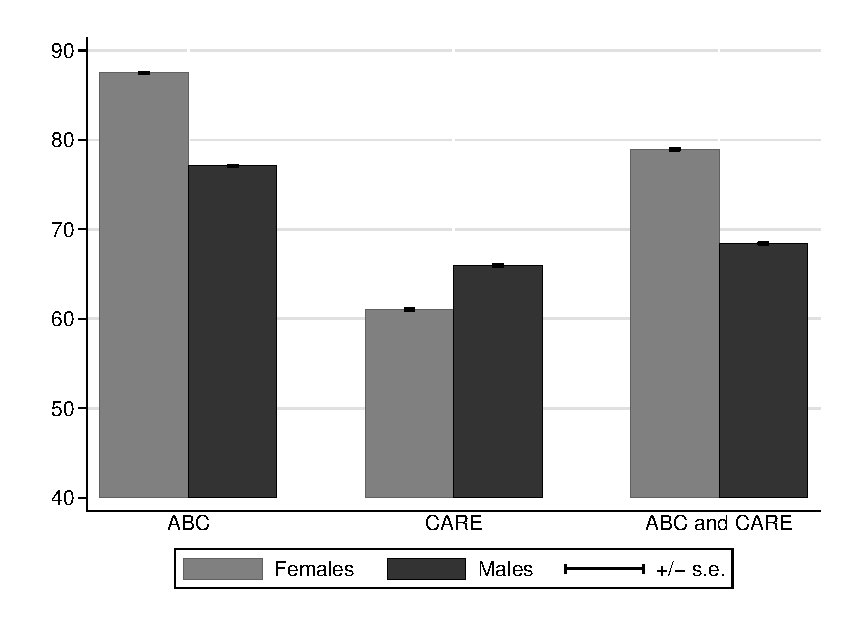
\includegraphics[width=\textwidth]{output/itt_noctrl_all.eps}
\end{subfigure}%
\begin{subfigure}[h]{0.4\textwidth}
	\centering
	\caption{Treatment vs. Next Best, Significant at 10\% Level} \label{fig:ppositive10}
		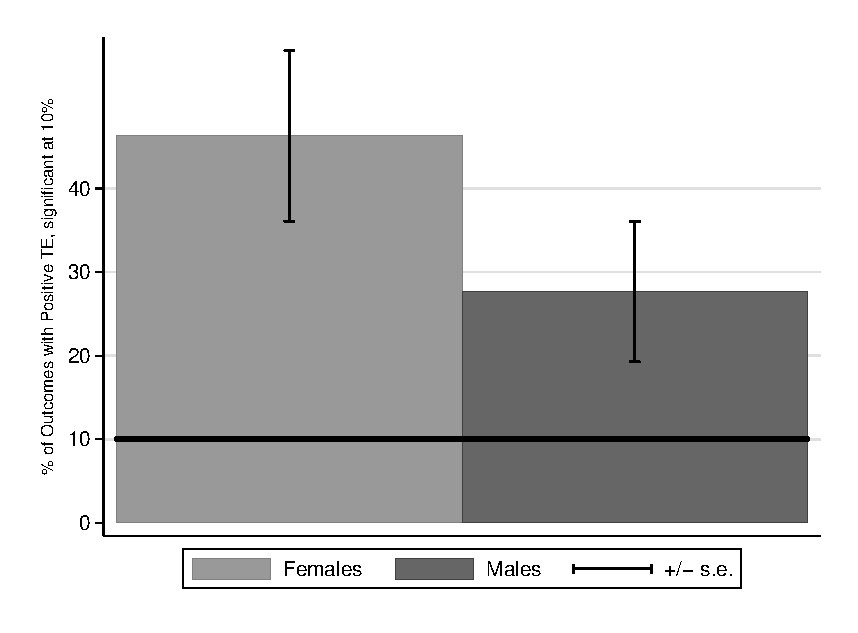
\includegraphics[width=\textwidth]{output/itt_noctrl_all_sig10.eps}
\end{subfigure}
\begin{subfigure}[h]{0.4\textwidth}
		\centering
		\caption{ Treatment vs. Stay at Home} \label{fig:ppositivehome}
		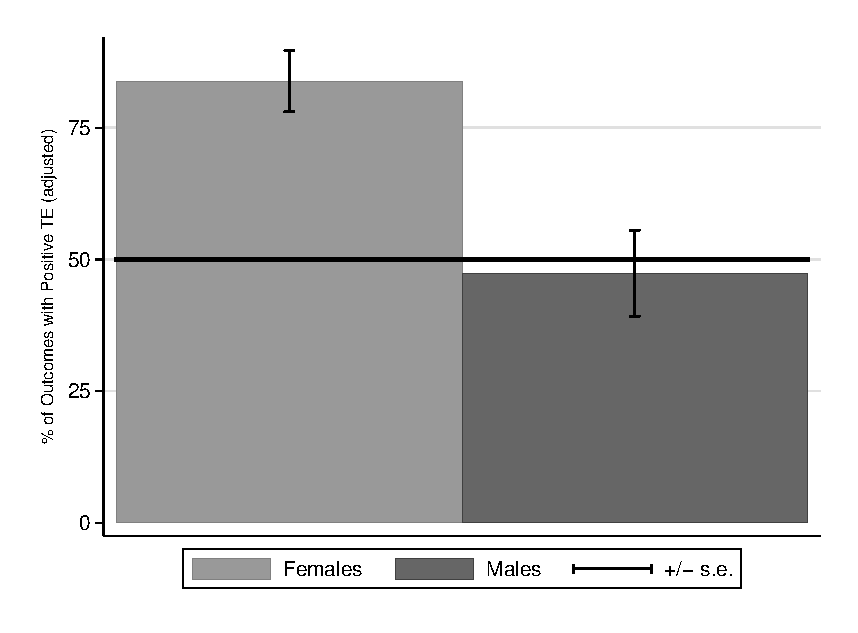
\includegraphics[width=\textwidth]{output/epan_ipw_p0_all.eps}
\end{subfigure}%
\begin{subfigure}[h]{0.4\textwidth}
	\centering
	\caption{Treatment vs. Alternative Childcare} \label{fig:ppositivealternative}
		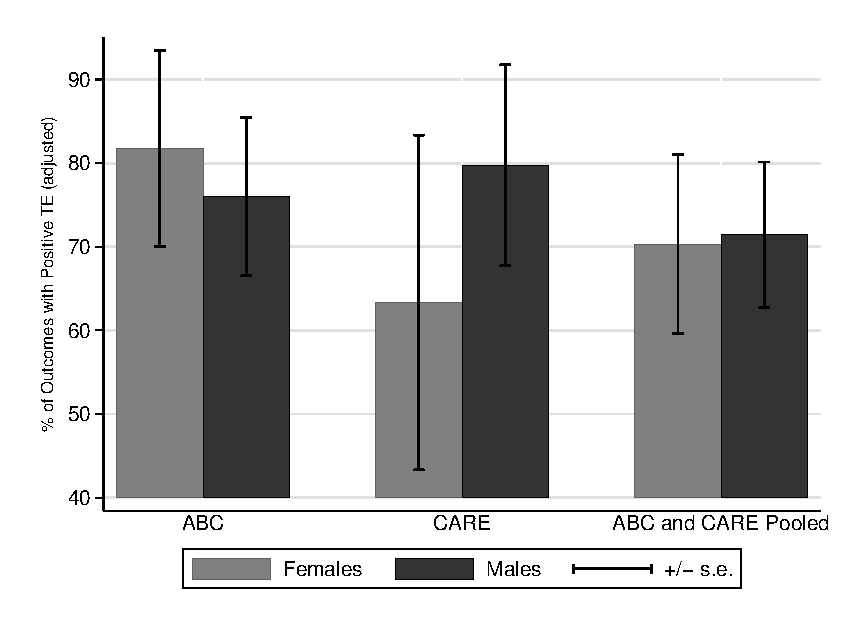
\includegraphics[width=\textwidth]{output/epan_ipw_p1_all.eps}
\end{subfigure}
\scriptsize \justify
Note: Panel (a) displays the percentage of outcomes displaying a positive treatment effect, comparing treatment to the next best option. Panel (b) displays the percentage of outcomes displaying a positive and statistically significant treatment effect (10\% significance level). Panel (c) displays the percentage of outcomes with a positive treatment effect, comparing treatment to staying at home. Panel (d) displays the percentage of outcomes with a positive treatment effect, comparing treatment to alternative childcare arrangements. Standard errors are based on the empirical bootstrap distribution. For Panel (b) we perform a ``double bootstrap'' procedure to first determine significant treatment effects at $10\%$ level and then calculate the standard error of the count.\\
\end{sidewaysfigure}

